     
      \subsubsection{Sensor de rotação (Efeito Hall)}
	
	O sensor escolhido foi o US1881 \textit{Hall Latch} – \textit{High Sensitivity} da Melexis
	(\textit{Microeletonic Integrated Systems}), que é um sensor
	digital disponível na loja virtual SparkFun a U\$ 0,95 (este valor não considera as taxas de envio). Devido à sua larga
	faixa de operação de tensão (VDD) e temperatura, esse sensor é adequado para a aplicação proposta \cite{melexis}.
	
	O sensor detecta a presença de polos magnéticos. Existem dois tipos de encapsulamentos, cujas lógicas de funcionamento
	são inversas e são apresentadas a seguir:
	
	\begin{figure}[!htbp]
	  \centering
	  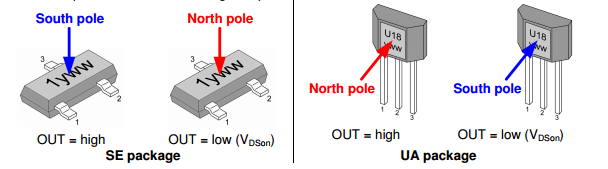
\includegraphics[scale=0.4]{editaveis/figuras/encapsulamento_sensor_efeito_hall}
	  \caption[Tipos de encapsulamento do sensor de efeito Hall]{Tipos de encapsulamento do sensor de efeito Hall \cite{melexis}.}
	  \label{encapsulamento_sensor_efeito_hall}
	\end{figure}
	
	\begin{figure}[!htbp]
	  \centering
	  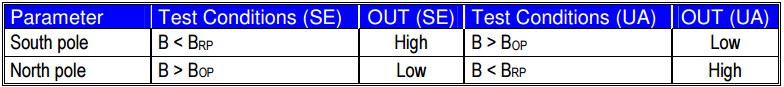
\includegraphics[scale=0.5]{editaveis/figuras/funcionamento_sensores_encapsulamento}
	  \caption[Lógica de funcionamento dos sensores considerado os encapsulamentos]
	  {Lógica de funcionamento dos sensores considerado os encapsulamentos (T = $-40^\circ\mathrm{C}$ a $150^\circ\mathrm{C}$, VDD = 3,5V a 24V) \cite{melexis}.}
	  \label{funcionamento_sensores_encapsulamento}
	\end{figure}
	
	Onde:
	
	\begin{itemize}
	 \item $B_{op}$ = Densidade de fluxo magnético aplicado no lado que tem a marca do encapsulamento que liga o condutor de saída.
	 \item $B_{rp}$ = Densidade de fluxo magnético aplicado no lado que tem a marca do encapsulamento que desliga o condutor de saída.
	\end{itemize}
	
	Abaixo é apresentada uma tabela com a os valores máximos suportados de diversos parâmetros 
	(informações necessárias para a estimação de consumo energético do sistema):
	
	\begin{figure}[!htbp]
	  \centering
	  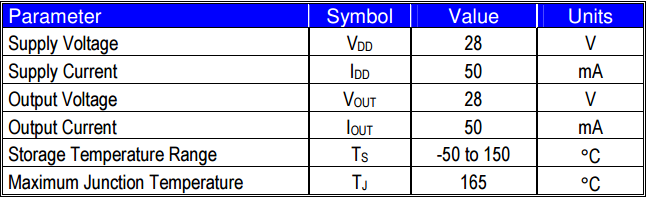
\includegraphics[scale=0.5]{editaveis/figuras/sensor_rotacao_max_valores}
	  \caption[Máximos valores suportados pelo sensor de rotação.]
	  {Máximos valores suportados pelo sensor de rotação \cite{melexis}.}
	  \label{sensor_rotacao_max_valores}
	\end{figure}
	
	Deve-se adquirir o sensor o qual tem o sufixo $\mathrm{L}$, uma vez que esse é o tipo que suporta a maior variação de
	temperatura: $-40^\circ\mathrm{C}$ a $150^\circ\mathrm{C}$ \cite{melexis}.
	
	As tabelas com as descrições/especificações do sensor são apresentadas abaixo:
	
	\begin{figure}[!htbp]
	  \centering
	  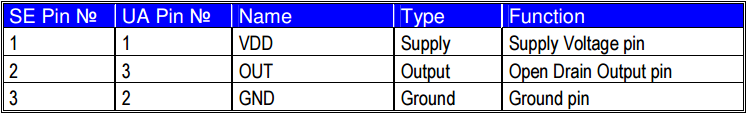
\includegraphics[scale=0.5]{editaveis/figuras/sensor_rotacao_pinagem}
	  \caption[Pinagem e função dos pinos do sensor de rotação]
	  {Pinagem e função dos pinos do sensor de rotação \cite{melexis}.}
	  \label{sensor_rotacao_pinagem}
	\end{figure}
	
	\begin{figure}[!htbp]
	  \centering
	  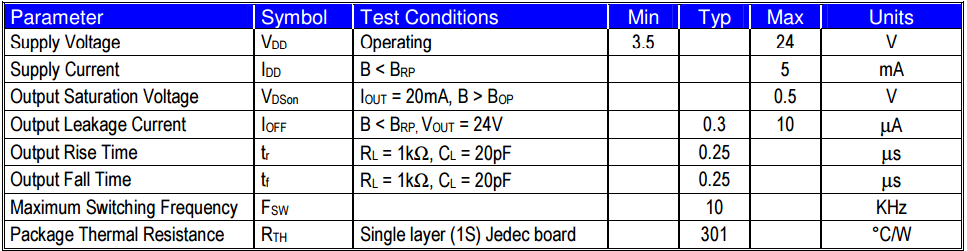
\includegraphics[scale=0.4]{editaveis/figuras/sensor_rotacao_spec_eletrica}
	  \caption[Pinagem e função dos pinos do sensor de rotação]
	  {Pinagem e função dos pinos do sensor de rotação \cite{melexis}.}
	  \label{sensor_rotacao_spec_eletrica}
	\end{figure}
	
	\begin{figure}[!htbp]
	  \centering
	  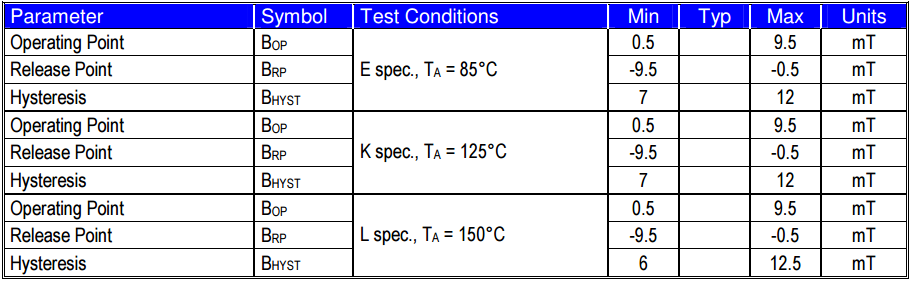
\includegraphics[scale=0.5]{editaveis/figuras/sensor_rotacao_spec_mag}
	  \caption[Especificações elétricas do sensor de rotação]
	  {Especificações elétricas do sensor de rotação \cite{melexis}.}
	  \label{sensor_rotacao_spec_mag}
	\end{figure}
	
	As figuras ~\ref{sensor_rotacao_idd_vs_vdd} e ~\ref{sensor_rotacao_vdd_vs_temperatura} apresentam dois gráficos
	de performance do sensor.
	
	\begin{figure}[!htbp]
	  \centering
	  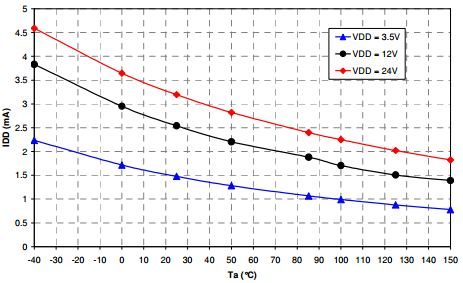
\includegraphics[scale=0.5]{editaveis/figuras/sensor_rotacao_idd_vs_vdd}
	  \caption[Sensor de rotação -  IDD vs VDD]
	  {Sensor de rotação -  IDD vs VDD \cite{melexis}.}
	  \label{sensor_rotacao_idd_vs_vdd}
	\end{figure}
	
	\begin{figure}[!htbp]
	  \centering
	  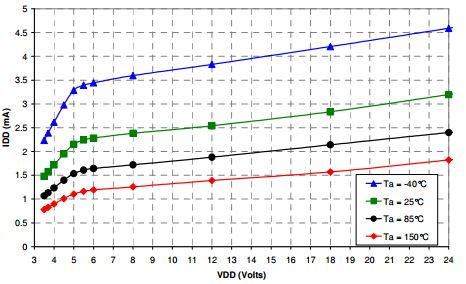
\includegraphics[scale=0.5]{editaveis/figuras/sensor_rotacao_vdd_vs_temperatura}
	  \caption[Sensor de rotação -  VDD vs Temperatura]
	  {Sensor de rotação -  VDD vs Temperatura \cite{melexis}.}
	  \label{sensor_rotacao_vdd_vs_temperatura}
	\end{figure}
	
	Para medir a velocidade de rotação da turbina, pretende-se elaborar uma montagem como a mostrada a seguir:
	 
	\begin{figure}[!htbp]
	  \centering
	  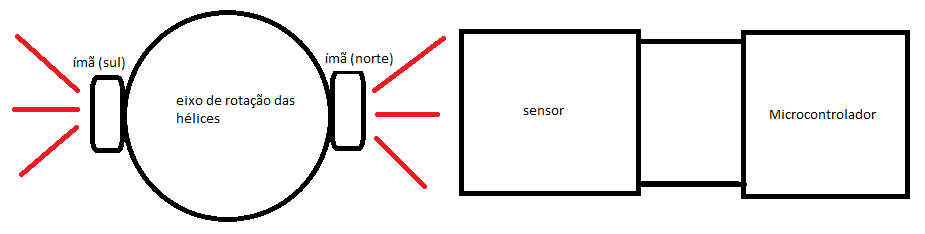
\includegraphics[scale=0.4]{editaveis/figuras/sensor_rotacao_monitoramento_velocidade}
	  \caption[Esquema simplificado de funcionamento do monitoramento da velocidade do eixo]
	  {Esquema simplificado de funcionamento do monitoramento da velocidade do eixo.}
	  \label{sensor_rotacao_monitoramento_velocidade}
	\end{figure}
	
	Uma vez que o sinal é digital, não há necessidade de filtragem do sinal, basta aplicar uma tensão VDD que seja suportada
	pelo microcontrolador (5V por exemplo).
	
	\begin{figure}[!htbp]
	  \centering
	  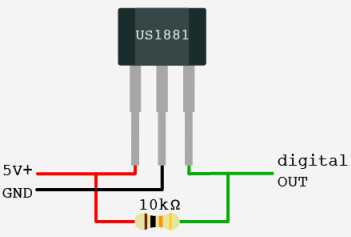
\includegraphics[scale=0.4]{editaveis/figuras/sensor_rotacao_conexao}
	  \caption[Esquema de conexão do sensor de rotação]
	  {Esquema de conexão do sensor de rotação. \footnotemark}
	  \label{sensor_rotacao_conexao}
	\end{figure}
	\footnotetext{Disponível em: <http://bildr.org/2011/04/various-hall-effect-sensors/>.}
	
	O algoritmo para determinar a velocidade de rotação das hélices deve, portanto, avaliar a frequência em que a saída do
	sensor apresenta-se em nível lógico alto (borda de subida) ou baixo (borda de descida) e com base nisso, efetuar o
	cálculo da velocidade (rpm, por exemplo).